\documentclass[11pt,letterpaper]{article}
\usepackage[T1]{fontenc}
\usepackage[utf8]{inputenc}
\usepackage{helvet}
\renewcommand{\familydefault}{\sfdefault}
\usepackage[margin=0.72in,headheight=14pt,footskip=25pt]{geometry}
\usepackage{graphicx,array,tabularx,colortbl,xcolor,enumitem,fancyhdr,amsmath}
\usepackage[hidelinks]{hyperref}
\hypersetup{pdftitle={Mothership Irrigation capacity estimates},pdfsubject={Fast preliminary estimates for the soft capsule airship},pdfauthor={}}
\definecolor{tablehead}{HTML}{E8EDF0}
\definecolor{tableline}{HTML}{D9D9D9}
\definecolor{muted}{HTML}{555555}
\setlength{\parindent}{0pt}
\setlength{\parskip}{7pt}
\renewcommand{\arraystretch}{1.28}
\setlength{\tabcolsep}{7pt}
\arrayrulecolor{tableline}
\setlist[itemize]{leftmargin=17pt,itemsep=3pt,topsep=4pt,parsep=0pt}
\pagestyle{fancy}
\fancyhf{}
\renewcommand{\headrulewidth}{0pt}
\renewcommand{\footrulewidth}{0pt}
\fancyfoot[L]{\footnotesize\color{muted}Fast preliminary estimates \quad 12 October 2026}
\fancyfoot[R]{\footnotesize\thepage}
\newcommand{\sectiontitle}[1]{\par\vspace{8pt}{\large\bfseries #1}\par\vspace{3pt}}
\newcolumntype{Y}{>{\raggedright\arraybackslash}X}
\newcolumntype{C}[1]{>{\centering\arraybackslash}p{#1}}
\begin{document}

{\fontsize{23}{27}\selectfont\bfseries Mothership Irrigation\par}
{\fontsize{17}{21}\selectfont Capacity estimates\par}
\vspace{5pt}
{\bfseries Fast preliminary estimates}\hfill 12 October 2026

These are fast estimates for exploring the scale of the \textbf{C soft capsule airship}. Component weights are rough planning allowances, supported by a few published hardware references. They have not been measured or validated as a complete aircraft.

An \textbf{8 m long and 4 m wide} envelope gives an initial budget for approximately \textbf{10--20 litres} of liquid. Carrying around \textbf{50 litres} moves the concept toward a \textbf{10 m long and 5 m wide} envelope. Controlling buoyancy as liquid is dispensed remains unresolved.

\begin{center}
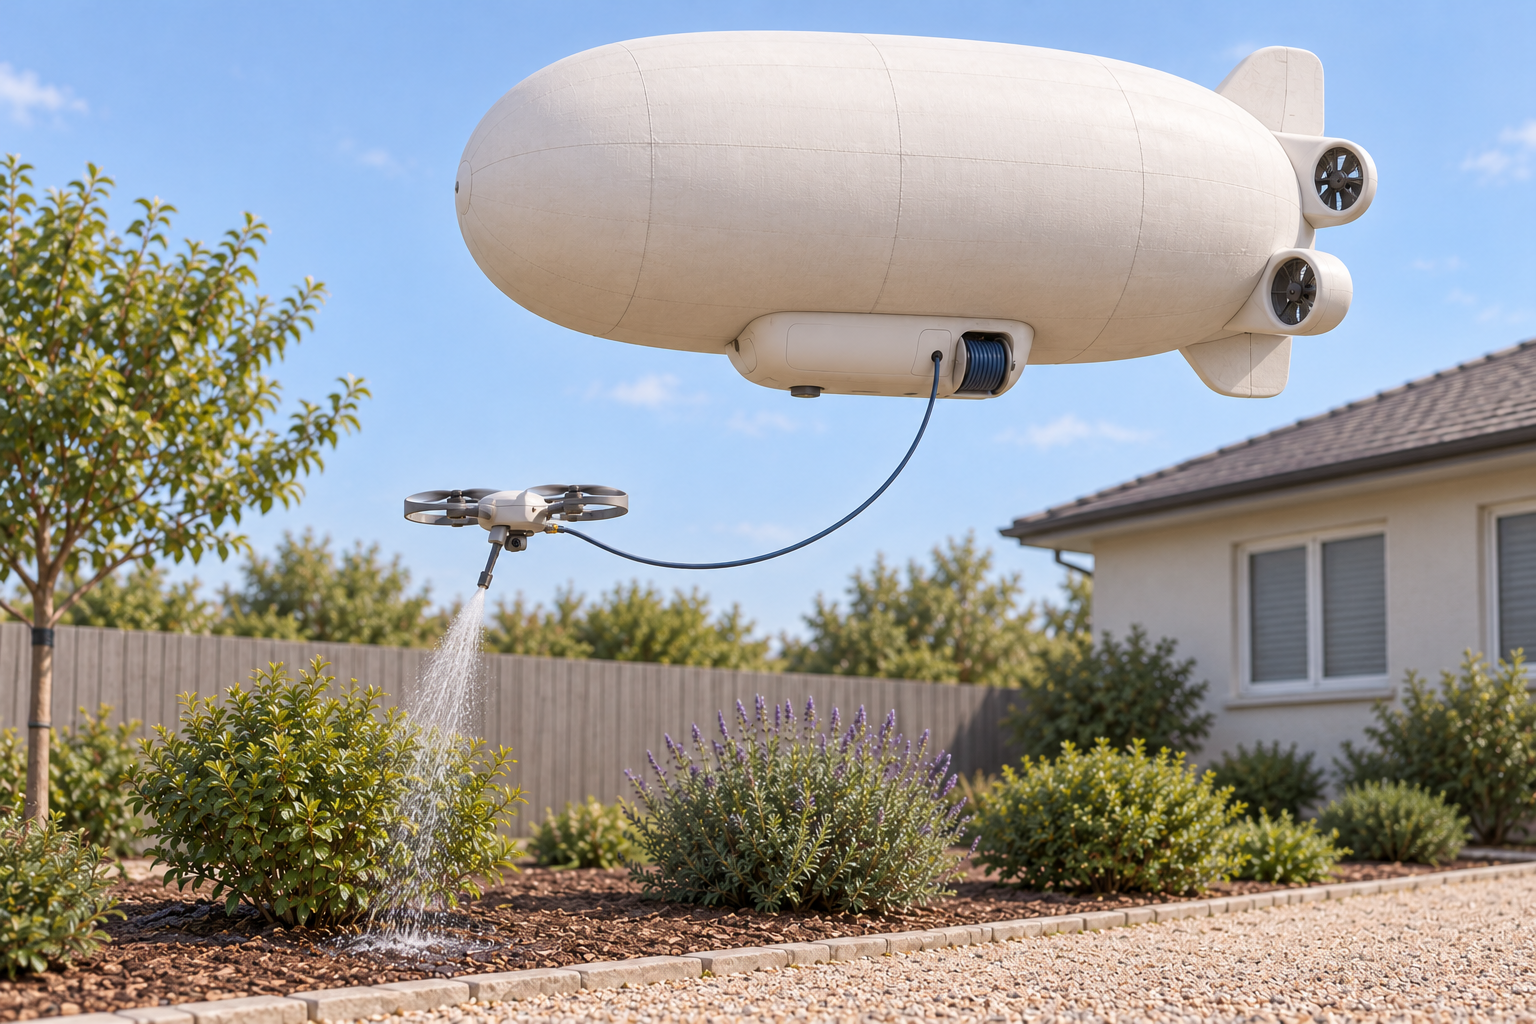
\includegraphics[width=0.72\textwidth]{illustrations/residential-c-soft-capsule-v3.png}\\[3pt]
{\small\color{muted}C is the visual basis. The illustration does not establish dimensions or hardware performance.}
\end{center}

\sectiontitle{Size and liquid capacity}
\begin{tabularx}{\textwidth}{|>{\raggedright\arraybackslash}p{1.52in}|C{1.35in}|Y|}
\hline
\rowcolor{tablehead}\textbf{Envelope size} & \textbf{Equipment mass} & \textbf{Total liquid budget}\\
\hline
$5 \times 2.5 \times 2.5$ m & 28--30 kg & No capacity with this package\\
\hline
$6 \times 3 \times 3$ m & 32--34 kg & No capacity with this package\\
\hline
$7 \times 3.5 \times 3.5$ m & 37--40 kg & 0--5 L\\
\hline
$\mathbf{8 \times 4 \times 4}$ \textbf{m} & \textbf{43--46 kg} & \textbf{10--20 L}\\
\hline
$10 \times 5 \times 5$ m & 61--66 kg & Approximately 40--60 L\\
\hline
$12 \times 6 \times 6$ m & 86--94 kg & Approximately 90--130 L\\
\hline
\end{tabularx}

{\small Dimensions are length, width and height of the gas envelope, excluding fins and the service pod. Equipment mass excludes helium and tank contents. Capacity includes a 15\% sizing allowance. Ranges reflect an oval versus a fuller capsule contour, rather than a statistical confidence interval.}

\newpage
\sectiontitle{Parts budget for the 8 metre version}
The envelope is approximately $8 \times 4 \times 4$ m, with 67--84 m$^3$ of outer volume. Two small drones are included, one working and one spare. The liquid load is additional to the equipment masses below.

\begin{tabularx}{\textwidth}{|Y|C{1.20in}|}
\hline
\rowcolor{tablehead}\textbf{Component} & \textbf{Estimated mass}\\
\hline
Fabric envelope including seams & 20--23 kg\\
\hline
Fins, attachments, valves and pressure-control hardware & 2.0 kg\\
\hline
Service pod and supporting frame & 3.0 kg\\
\hline
Thrusters, guards and motor controllers & 3.0 kg\\
\hline
Mothership battery of approximately 1 kWh & 5.0 kg\\
\hline
Computer, navigation and obstacle sensors & 1.2 kg\\
\hline
Empty liquid containers & 1.5 kg\\
\hline
Pumps, liquid valves and filters & 1.5 kg\\
\hline
Hose, fluid in the hose and powered reel & 1.5 kg\\
\hline
Two drones with batteries, cameras, guards and nozzles & 3.0 kg\\
\hline
Docking hardware, wiring and miscellaneous parts & 1.5 kg\\
\hline
\rowcolor{tablehead}\textbf{Total equipment mass} & \textbf{43--46 kg}\\
\hline
\end{tabularx}

The fabric has approximately \textbf{86--101 m$^2$ of surface}. At 200 g/m$^2$ plus a 15\% seam allowance, it contributes approximately 20--23 kg. This is a material mass reference, not a selected envelope specification [2].

The battery allocation has a practical reference: two 488.4 Wh commercial packs provide 976.8 Wh and weigh 4.92 kg [3]. This does not establish flight duration. Other part weights remain approximate allocations, including propulsion, pressure control and sensor integration.

\sectiontitle{Assumptions behind the calculation}
\begin{itemize}
\item Dry air at 35 $^\circ$C and 101.325 kPa, with helium at the same temperature; small envelope overpressure neglected.
\item Approximately 95\% helium volume and 5\% ambient-air ballonet space. The internal air is accounted for in the lifting calculation.
\item Water and dilute mixtures approximated as 1 kg/L. All tank contents share the liquid budget, including treatment, feed and rinse liquid.
\item Envelope material at 200 g/m$^2$, plus 15\% for seams and local reinforcement. Separate fittings and fins are counted in the parts table.
\item Approximately 15 m of lightweight hose; a 4 mm internal diameter holds about 0.19 L, already counted in the hose allocation.
\item Fifteen per cent of net lifting capacity is kept outside the planned equipment and liquid budget for sizing uncertainty. Actual flight still needs a trim strategy.
\end{itemize}

{\small The calculated net helium lifting capacity is approximately 63--79 kg, after accounting for helium's own weight. Deducting equipment and the sizing allowance leaves the 10--20 L liquid budget [1].}

\newpage
\sectiontitle{What happens as the tanks empty}
If the airship starts neutrally buoyant and dispenses 10 litres of water, it becomes approximately \textbf{10 kg lighter}. The resulting upward imbalance is about \textbf{98 N}. At 20 litres dispensed, it is about \textbf{196 N}.

The initial lifting budget therefore does not establish usable operating capacity. The system needs a controlled ground tether, sufficient downward or vectorable thrust, or an engineered buoyancy and ballast system. Horizontal steering fans alone do not demonstrate vertical control.

Ordinary small-pressure ballonets cannot simply be assumed to offset a 10--20 kg payload change. Replacing that mass with ambient air would require roughly 9--17 m$^3$ of air at these conditions, with substantial helium compression or gas-volume change. Deployment and recovery of the drones also change the supported load.

\sectiontitle{Sensitivity to envelope material}
Keeping the 8 m dimensions and other assumptions unchanged gives:

\begin{tabularx}{\textwidth}{|p{2.15in}|Y|}
\hline
\rowcolor{tablehead}\textbf{Fabric mass per square metre} & \textbf{Estimated liquid budget}\\
\hline
150 g/m$^2$ & 15--26 L\\
\hline
200 g/m$^2$ & 10--20 L\\
\hline
300 g/m$^2$ & 1--9 L\\
\hline
\end{tabularx}

{\small These are sensitivity cases, not validated fabric choices. Each additional kilogram of equipment or ballast removes approximately one litre of water-like capacity. Wind control, wet fabric and environmental conditions may reduce the available budget further.}

\sectiontitle{Working reference for further discussion}
Use \textbf{C as the visual basis}, an \textbf{8 m by 4 m envelope} as the first sizing reference, and \textbf{10 litres} as the conservative liquid target. A fuller capsule shape may increase that budget toward 20 litres, subject to actual component masses and the buoyancy-control design.

This scale suits targeted plant care. Large-volume irrigation would require a substantially larger airship or liquid supplied from the ground. These remain \textbf{fast preliminary estimates}; they are a basis for discussion and refinement.

\sectiontitle{Calculation and reference checks}
At the assumed temperature and pressure, helium provides approximately 0.987 kg of net lifting capacity per cubic metre of helium [1]. Outer volumes use an oval ellipsoid and a capsule with hemispherical ends. The estimate is:
\[
m_{\mathrm{liquid}} \approx 0.85(0.95V)(0.987)-m_{\mathrm{equipment}},
\]
where $V$ is outer volume in m$^3$ and masses are in kg. Helium weight is already deducted in 0.987 and is not subtracted again.

{\small
[1] \href{https://www.grc.nasa.gov/www/k-12/WindTunnel/Activities/ArchAnswer5.html}{NASA buoyancy example} and \href{https://www1.grc.nasa.gov/beginners-guide-to-aeronautics/gas-density/}{NASA gas density explanation}.\\[3pt]
[2] \href{https://pmc.ncbi.nlm.nih.gov/articles/PMC6165535/}{Airship envelope material study}, reporting 200 g/m$^2$ multilayer material.\\[3pt]
[3] \href{https://www.grepow.com/uav-battery/tattu-6s-lipo-drone-battery.html}{Grepow Tattu battery specifications}, listing 488.4 Wh at 2.46 kg per pack.\\[3pt]
Further assumptions and component references are retained in the project note \texttt{CAPACITY\_ESTIMATE.md}.
}
\end{document}
